\chapter{Behavior Mapping}

\section{Overview of Behavior Mapping}
Our ultimate goal is to have a fine-grained categorization of the behaviors observed during dormancy. Thus, it is not sufficient to outline experiments and construct the sets $\MicroActivity$ and $\MacroActivity$. Behavior mapping stage is the most critical and novel part of the pipeline, and in this stage, we discover and predict stereotypical behaviors by mapping each frame in the sets $\MicroActivity$.

Behavior mapping stage starts by generating low dimensional behavioral embeddings from high dimensional behavioral matrix $\V{\hat{W}}$, but only the rows corresponding to the $\MicroActivity$ are included in the mapping.
Rest of the frames, namely the $\Quiescence$ set and $\MacroActivity$ set directly assigned to quiescent and moving categories.
In the Section~\ref{section:behavioral-embeddings}, behavioral embedding generation is discussed in detail, including supervised, semi-supervised and unsupervised approaches.
We use semi-supervised pair UMAP embeddings, described in the Section~\ref{section:pair-embeddings}, to map frames to behaviors.

The next step is a novel nearest neighbor analysis in the generated low dimensional behavioral spaces, as we detail in the Section~\ref{section:nearest-neighbors-classification}.
Nearest neighbor analysis consists of several parts.
First one is the computation of the behavioral weights (Section ~\ref{section:behavioral-weights}). Next, we combine behavioral weights provided by each ``view'', i.e., annotated experiment by forming a committee (Section~\ref{section:committee-by-voting}).
Finally post-processing is described in the Section~\ref{section:postprocessing-predictions}.

\section{Behavioral Embeddings}\label{section:behavioral-embeddings}
The dynamic postural features are able to capture many different timescales, however their high-dimensional structure makes it challenging to directly exploit behavioral representations in analysis, learning, and visualization.
For example, the behavioral representation matrix ($\V{\hat{W}}$) computed from dynamic postural features ($\V{W}$) with $20$ spatio-temporal features and $25$ timescales (i.e., frequency channels) has $20 \times 25 {=} 500$ columns.
Since the correlation between different spatio-temporal features (e.g., distance between head and proboscis and cartesian pose values of proboscis) and different timescales are often strong (see Figure~\ref{figure:correlations-btw-features}), one may expect that the topological structure of the high dimensional behavioral representations ($\V{\hat{W}}$) can be accurately represented in a lower dimensional space.
Therefore, we would like to find a low-dimensional embedding that captures the important features of the dataset.
The embedding we compute should minimize local distortions, since trajectories pause near a repeatable position whenever a particular stereotyped behavior is observed \citep{berman_mapping_2014, deangelis_manifold_2019, ali_timecluster_2019}.

\begin{figure}[ht!]
	\centering
	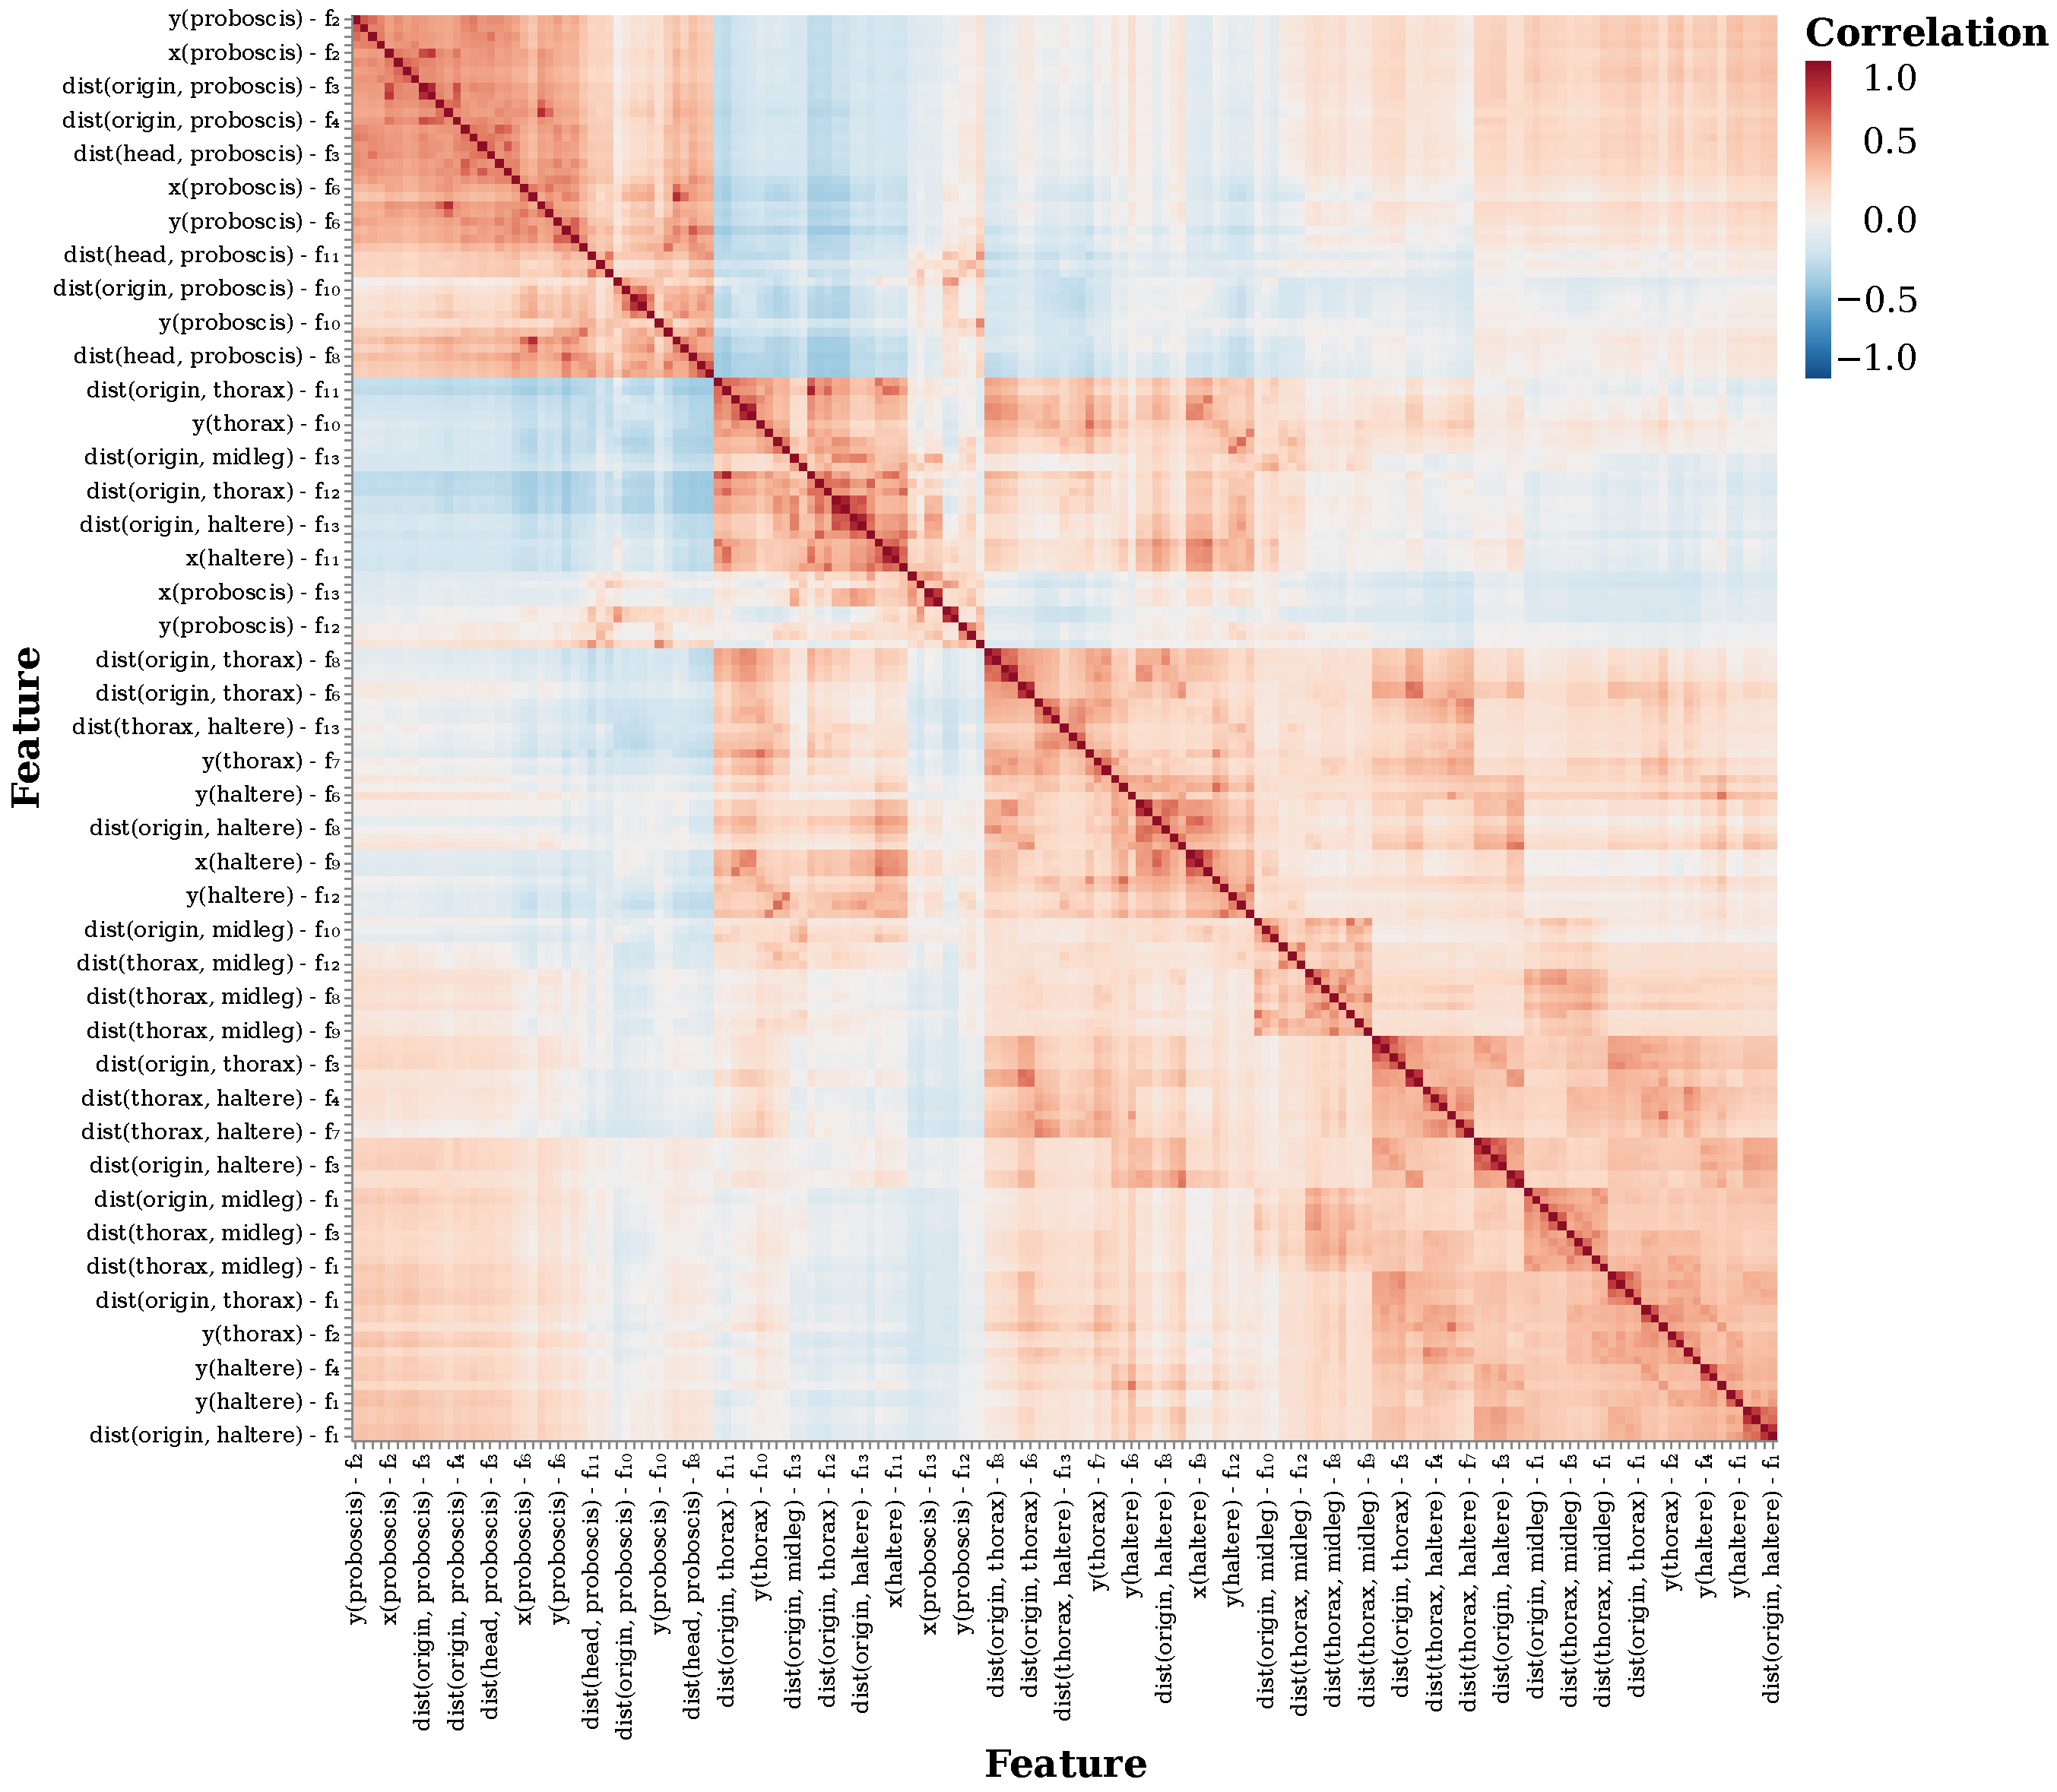
\includegraphics[width=0.70\linewidth]{figures/FeatureCorrelations-FlyF1DAnn-XY_labels.pdf}
	\caption[Spearman's correlation coefficient between each feature value of behavioral representations.]{Spearman's correlation coefficient between each feature value of behavioral representations. Features are clustered and grouped based on the absolute value of the correlation values. Frequency channels $f_1, \cdots, f_20$ are dyadically spaced between $1$ Hz and $20$ Hz. \label{figure:correlations-btw-features}}
\end{figure}

Many dimensionality reduction algorithms seek to preserve the pairwise distance structure among all the data samples, the well-known examples of such algorithms are PCA \citep{hotelling_analysis_1933}, and MDS \citep{kruskal_multidimensional_1964}.
Alternatively, some algorithms favor the preservation of local distances over global distance, such as UMAP (Uniform Manifold Approximation \& Projection) \citep{mcinnes_umap_2020} t-SNE \citep{maaten_visualizing_2008}, Laplacian Eigenmaps \citep{belkin_laplacian_2003} and LargeVis \citep{tang_visualizing_2016}.
The latter category of algorithms aims to achieve to preserve important local structures, and helps to improve classification performance when used in combination with learning algorithms where the function is only approximated locally, e.g., $k$-nearest neighbor classifier \citep{mcinnes_umap_2020}.
Similarly, it has been shown that manifold learning based dimensionality reduction algorithms can improve the clustering performance \citep{sainburg_parametric_2021}.
Moreover, the trade-off of preserving local distances over global distances does not introduce any significant disadvantages in the latter stages of the behavioral pipeline.

We use UMAP for its superior performance in many aspects.
\citet{mcinnes_umap_2020} demonstrates that a $k$-nearest neighbor classifier trained on UMAP embeddings achieves higher accuracy for large $k$ values, compared to PCA, t-SNE, LargeVis and Laplacian Eigenmaps since it captures non-local scales in a markedly effective way and local scales comparably or better.
Thus, it can be argued that UMAP has captured more of the global and topological structure of the benchmark datasets than its counterparts, t-SNE and LargeVis.
Another reason for choosing UMAP over other alternatives is that it tends to produce more stable embeddings.
It is capable of producing sub-sample embeddings which are very close to the full embedding even for sub-samples of $5\%$ of the dataset, outperforming the results of t-SNE and LargeVis.
Finally, computational performance of UMAP scales well with the number of samples, the embedding dimensionality and the data dimensionality, compared to t-SNE LargeVis, and Eigenmaps, resulting significantly lower run-times on various datasets such as  COIL-20 \citep{nene_columbia_1996}, Fashion-MNIST \citep{xiao_fashion-mnist_2017}, and GoogleNews \citep{mikolov_distributed_2013}.
Run-time performance of the dimensionality reduction algorithm is an important concern in the behavioral mapping pipeline, as the number of samples and the data dimensionality is often on the order of $10^6$ and $10^2$, respectively.

UMAP and other non-linear dimensionality reduction algorithms that attempt to use a mathematical structure akin to a $k$-nearest neighbor graph to approximate a manifold, follow a similar basic structure as below \citep{mcinnes_umap_2020}.
\begin{itemize} \item Graph Construction \begin{enumerate}
		      \item Construct a weighted $k$-nearest neighbor graph.
		      \item Apply some transformation on the edge weights to envelop local distances.
		      \item Deal with the incompatibility of the local metrics, i.e., disagreeing weights of the edges.
	      \end{enumerate}
	\item Graph Layout
	      \begin{enumerate}
		      \item Define an objective function that preservers desired characteristics of the $k$-nearest neighbor graph.
		      \item Compute a low dimensional representation by optimizing the defined objective function.
	      \end{enumerate}
\end{itemize}

A distance metric is needed to construct a $k$-nearest neighbor ($k$-NN) graph.
In our case, we normalized the feature matrices as described in Section~\ref{section:feature-normalization}, feature vector entries at each time step sum up to $1$, and therefore the feature vectors  can be considered as discrete probability distributions.
We use the Hellinger distance \citep{hellinger_neue_1909} to quantify the similarity between ``discrete probability distributions'' of features, which is given by
\begin{equation}\label{equation:hellinger-distance}
	\operatorname{Hellinger}(P,Q)={\frac {1}{\sqrt {2}}}\;{\sqrt {\sum _{i=1}^{k}({\sqrt {p_{i}}}-{\sqrt {q_{i}}})^{2}}}.
\end{equation}
Then, based on the Hellinger distances, UMAP constructs a weighted $k$-NN graph using nearest neighbor descent \citep{dong_efficient_2011}.
Then, the $k$-NN graph is modified by making edges directed and defining the new weights using local Riemannian metric of each data point.
After this step, there exist two edges with disagreeing weights between the nearest neighbors, as the local metrics differ.
UMAP combines those weights by using $t$-conorm and the resulting weight can be interpreted as the probability of at least one of the two directed edge to exist.

Finally, UMAP uses a force directed graph layout algorithm in low dimensional space where attractive and repulsive forces are defined based on the gradients, optimizing the edge-wise cross-entropy between the original weighted graph and equivalent weighted graph induced by the embeddings.
The algorithm proceeds by iteratively applying attractive and repulsive forces at each edge or vertex.
Since the ``true'' graph captures the topology of the source data, the approximated graph also matches the overall topology of the data, and thus produces a meaningful low dimensional representation.
A detailed mathematical and algorithmic description of the UMAP algorithm can be found in \citep{mcinnes_umap_2020}, and it is skipped here as it goes beyond the scope of this work.

\begin{comment}
\begin{algorithm}[!htbp]
	\caption{The main UMAP algorithm.}\label{alg:umap}
	\begin{algorithmic}[0]
		\setlength\baselineskip{18pt}
		\Function{UMAP}{$X$, $n$, $d$, min-dist, n-epochs}
		\State
		\State \# \textit{Construct the relevant weighted graph}
		\ForAll{$x \in X$}
		\State fs-set[$x$] $\gets$ \Call{LocalFuzzySimplicialSet}{$X$, $x$, $n$}
		\EndFor
		\State top-rep $\gets \bigcup_{x\in X} \textrm{fs-set}[x]$ \Comment{The probabilistic t-conorm is recommended.}
		\State
		\State \# \textit{Perform optimization of the graph layout}
		\State $Y \gets$ \Call{SpectralEmbedding}{top-rep, $d$}
		\State $Y \gets$ \Call{OptimizeEmbedding}{top-rep, $Y$, min-dist, n-epochs}
		\State \Return $Y$
		\EndFunction\vskip9pt
	\end{algorithmic}
\end{algorithm}
\end{comment}

The algorithm described above is an unsupervised method, but it can be easily extended to work in a supervised or semi-supervised manner.
Although we use a useful metric, e.g., Hellinger distance, defining the distance between a set of points, one can also define a simple metric for categorical values to extend UMAP further for supervised and semi-supervised cases.
We can obtain a second view on the source data by using a metric where distances for points in the same  and different categories as well as points without a category (for the semi-supervised case) are defined appropriately.
A straightforward and simple example would be defining distances as follows: 1 if the points are in the same category, 0 if the points are in different categories, 0.5 if either of the points is uncategorized.
One can combine weighted graphs constructed using the two distance metrics (local metrics and defined metric for categorical values), and arrive at a shared view on the data.
In the behavioral mapping pipeline, we benefit from unsupervised UMAP, and its supervised and semi-supervised extensions for different purposes.

The utilized behavioral embeddings fall into three different categories, namely ``disparate embeddings'', ``joint embeddings'' and ``pair embeddings'', detailed descriptions and their applications are described respectively in  Section~\ref{section:disparate-embeddings}, Section~\ref{section:joint-embeddings}, and  Section~\ref{section:pair-embeddings} respectively.

The resulting behavioral embedding
\begin{equation}
	\V{E}=\qmatrix{\V{e}_1, \cdots \V{e}_{F}} \in F \times N,
\end{equation}
is a low-dimensional representation of
\begin{equation}
	\mathrm{row}_{t_f} \V{\hat{W}} \in \mathbb{R}^{F \times \rbr{ N_S\card*{\mathcal{T}_S}}} \ \rbr{t_f \in \MicroActivity},
\end{equation}
where and $N << \rbr{ N_S\card*{\mathcal{T}_S}}$ and $F$ is the numbers of frames estimated as dormant and active, being equal to $\card{\MicroActivity}$.
Each frame $f$, corresponds to a time point $t_f\in \MicroActivity$.

\subsection{Disparate Embeddings}\label{section:disparate-embeddings}
UMAP may be used to embed high-dimensional behavioral representations of each experiment separately to obtain disparate behavioral embeddings. Treating each experiment separately is useful for several purposes.

For example, using supervised UMAP for annotated experiments, we can explore behavioral sub-categories in annotations as annotations are very high-level, biased and general categorization of behaviors. For instance, one annotation category, e.g., "grooming", can be consisted of two different clusters in the behavioral embedding space, corresponding to "grooming of head" and "grooming of abdomen" (see Figure~\ref{figure:supervised-disparate-zoomin-annotations}).
Defining very specific and low-level behavioral categories is not feasible and prone to error, a post-annotation analysis using disparate embeddings helps us to zoom in annotated behaviors.
Another scenario of benefiting disparate embeddings is using unsupervised UMAP for annotated and/or unannotated experiments separately.
We can visualize how behavioral repertoire is represented in the low dimensional embeddings space and analyze which features drives different regions and clusters of the behavioral embeddings (see Figure~\ref{figure:unsupervised-disparate-behavioral-regions}).

\begin{figure}[htb!]
	\centering
	\begin{subfigure}[b]{0.5\linewidth}
		\centering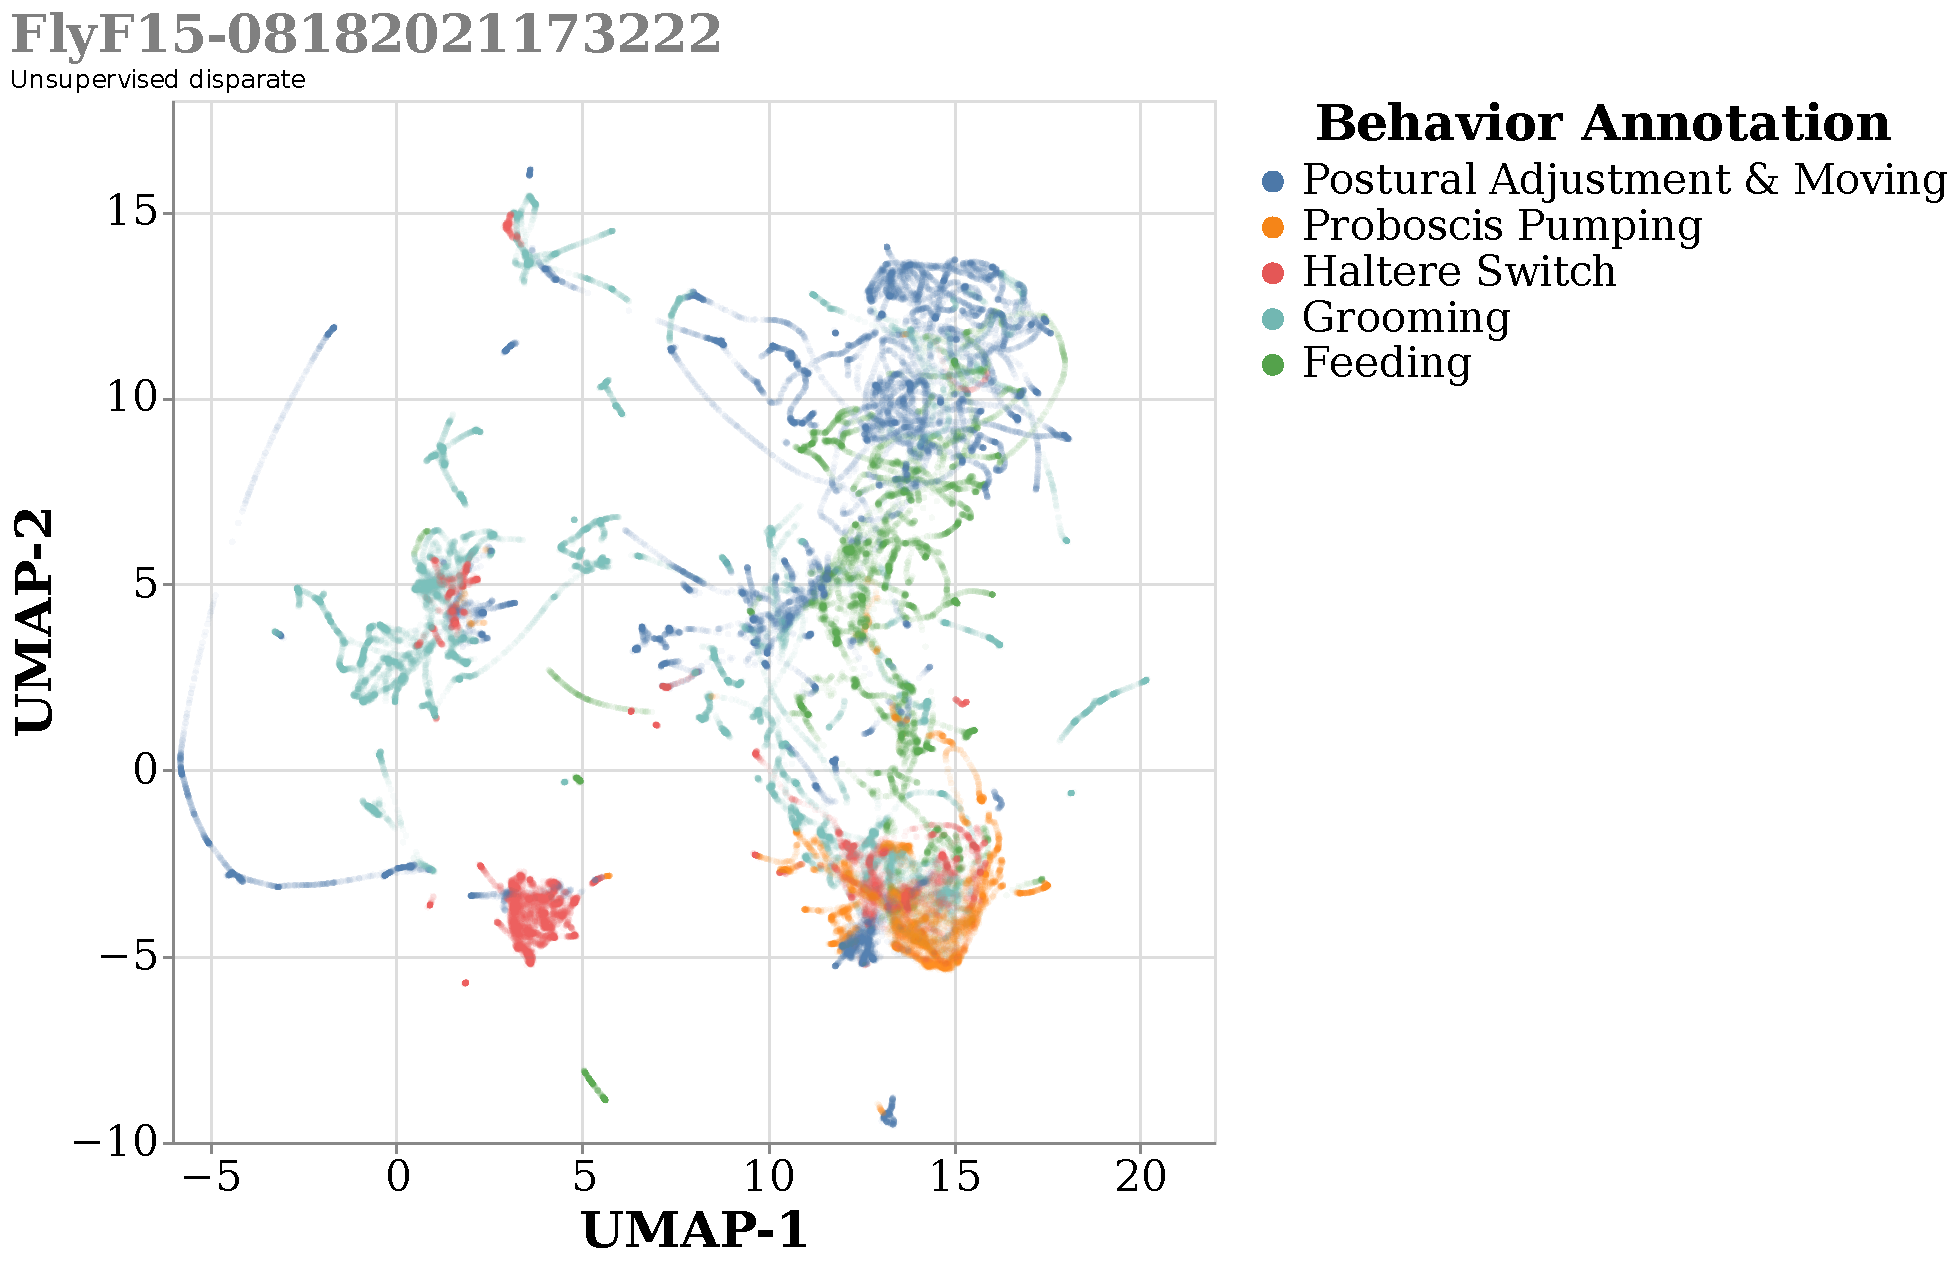
\includegraphics[height=5cm]{figures/FlyF15-08182021173222_UnsupervisedDisparateEmbedding.pdf}
		\caption{Unsupervised. \label{figure:unsupervised-disparate-behavioral-regions}}
	\end{subfigure}%
	\hfill
	\centering
	\begin{subfigure}[b]{0.5\linewidth}
		\centering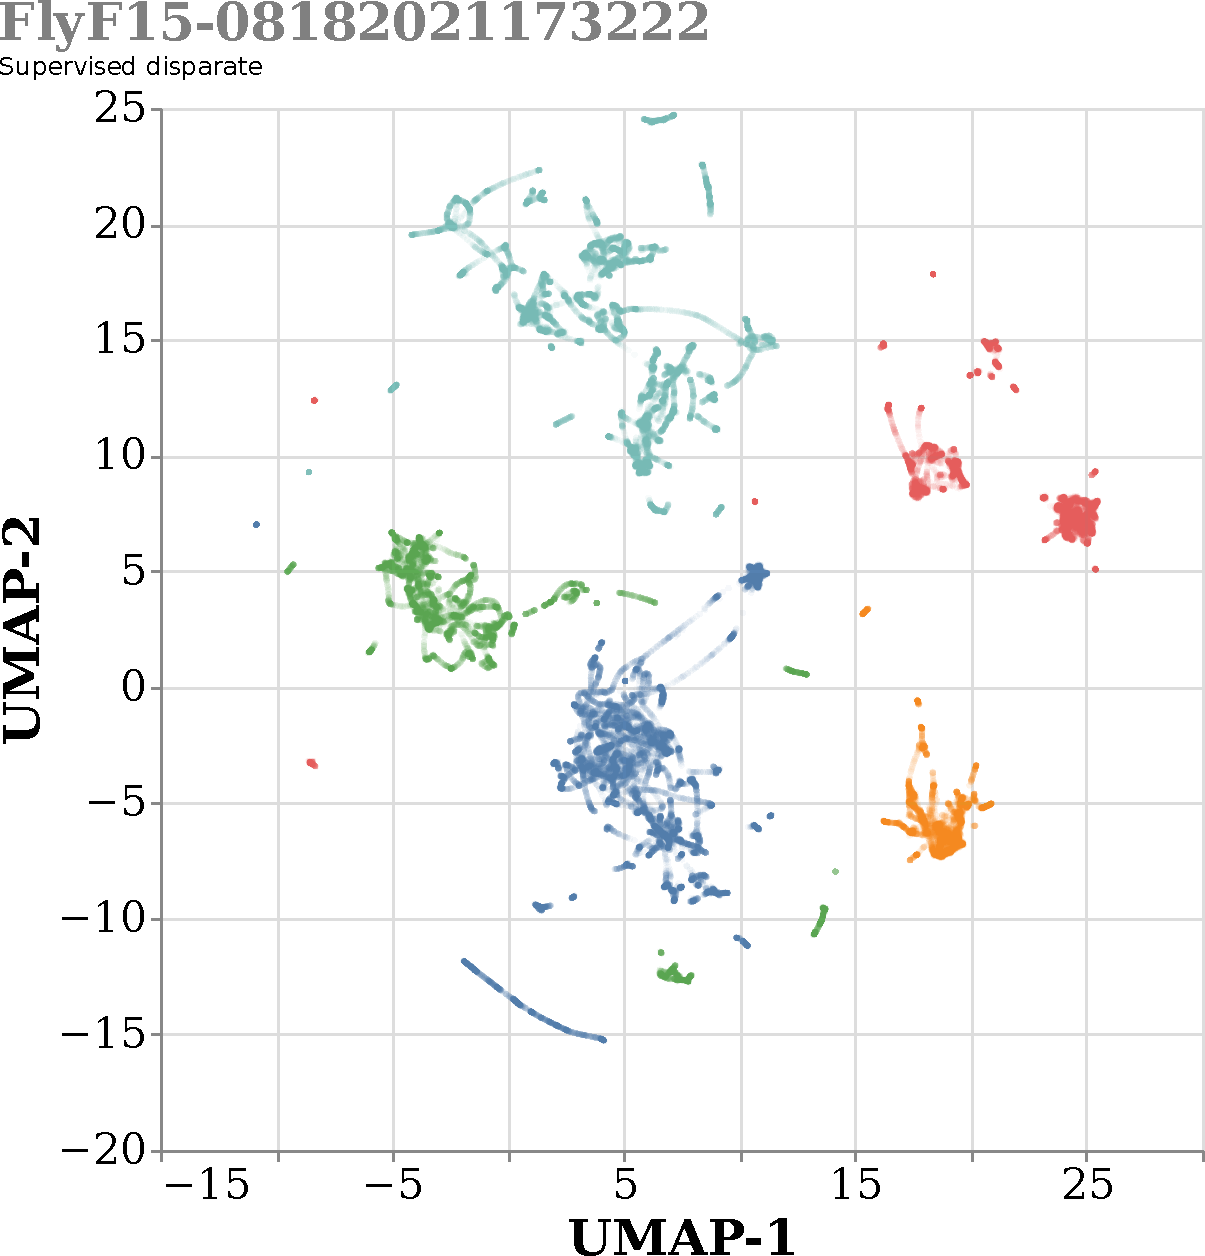
\includegraphics[height=5cm]{figures/FlyF15-08182021173222_SupervisedDisparateEmbedding.pdf}
		\caption{Supervised. \label{figure:supervised-disparate-zoomin-annotations}}
	\end{subfigure}%
	\caption[Supervised and unsupervised embeddings of FlyF15-08182021173222.]{Two-dimensional supervised and unsupervised behavioral embeddings of FlyF15-08182021173222. Both embeddings reveal variations within annotated behavioral categories.}
\end{figure}

\subsection{Joint Embeddings}\label{section:joint-embeddings}
Ideally, we would like to embed all experiments into a shared joint behavioral space, and using such an embedding would enable us to discover stereotypical and common behaviors among different flies.
However, we observed that this is only possible to a certain extent and such joint embeddings tend to not mix well as the number of experiments increases.
When we jointly compute a behavioral space using all available experiments,  the resulting embedding is usually not totally homogeneous in terms of flies and experiments.
We observed that similar behaviors might end up embedded in different regions, and multiple clusters consisting of highly similar behaviors emerges.

Especially for the joint treatment of annotated experiments, supervised UMAP fails to embed similar behaviors of different experiments closely and homogeneously.
There are many factors contributing to this impairment of supervised joint embeddings, such as behavioral variations among flies and experiments,  differences in orientation while exhibiting similar behaviors, and broad definitions of annotation categories.
Unless the number of jointly embedded experiments does not exceed several, unsupervised UMAP performs relatively well, and enables a fully unsupervised and unbiased analysis of behaviors.
We can exploit unsupervised joint behavioral embeddings for visualization purposes to discover how different feature combinations are exhibited, and density-based clustering to extract similar behavioral bouts.
However, utilizing unsupervised joint embeddings becomes problematic as the number of experiments increases, and behavioral space gets ``too crowded''.

\subsection{Pair Embeddings}\label{section:pair-embeddings}
Using disparate embeddings does not allow one to embed an annotated and an unannotated experiment into a joint behavioral space, and joint embeddings poorly blend different experiments in a shared space.
Instead, we propose a novel alternative approach to benefit from the semi-supervised dimensionality reduction capabilities of UMAP, while avoiding generating a hard-to-interpret embedding.
In this approach, namely semi-supervised pair embeddings, we compute a joint behavioral space for each annotated and unannotated pair, using the available annotations.
As a result, for $\Unann{R}$ unannotated experiments and  $\Unann{R}$ annotated experiments, a semi-supervised pair embedding will be generated for each $\Unann{R} \times \Ann{R}$ pair.

For a single unannotated experiment, a semi-supervised behavioral embedding for each annotated experiment provides different ``views''.
Especially when the behavioral repertoire of the annotated and the unannotated experiments are similar, the provided ``view'' turns out to be an accurate, easy-to-interpret low-dimensional representation of the exhibited behaviors of the unannotated experiment.
When the behavioral repertoire and/or feature distribution are dissimilar, the resulting embedding may not provide useful information about the unannotated experiment, but an advantage of this approach is that the other pair embeddings do not get distorted by poor matches.
As described in Section~\ref{section:nearest-neighbors-classification}, semi-supervised pair embeddings are utilized to predict behavioral categories of unannotated experiments by combining multiple view acquired from annotated ones.

\begin{figure}[htb!]
	\centering
	\begin{subfigure}[b]{0.5\linewidth}
		\centering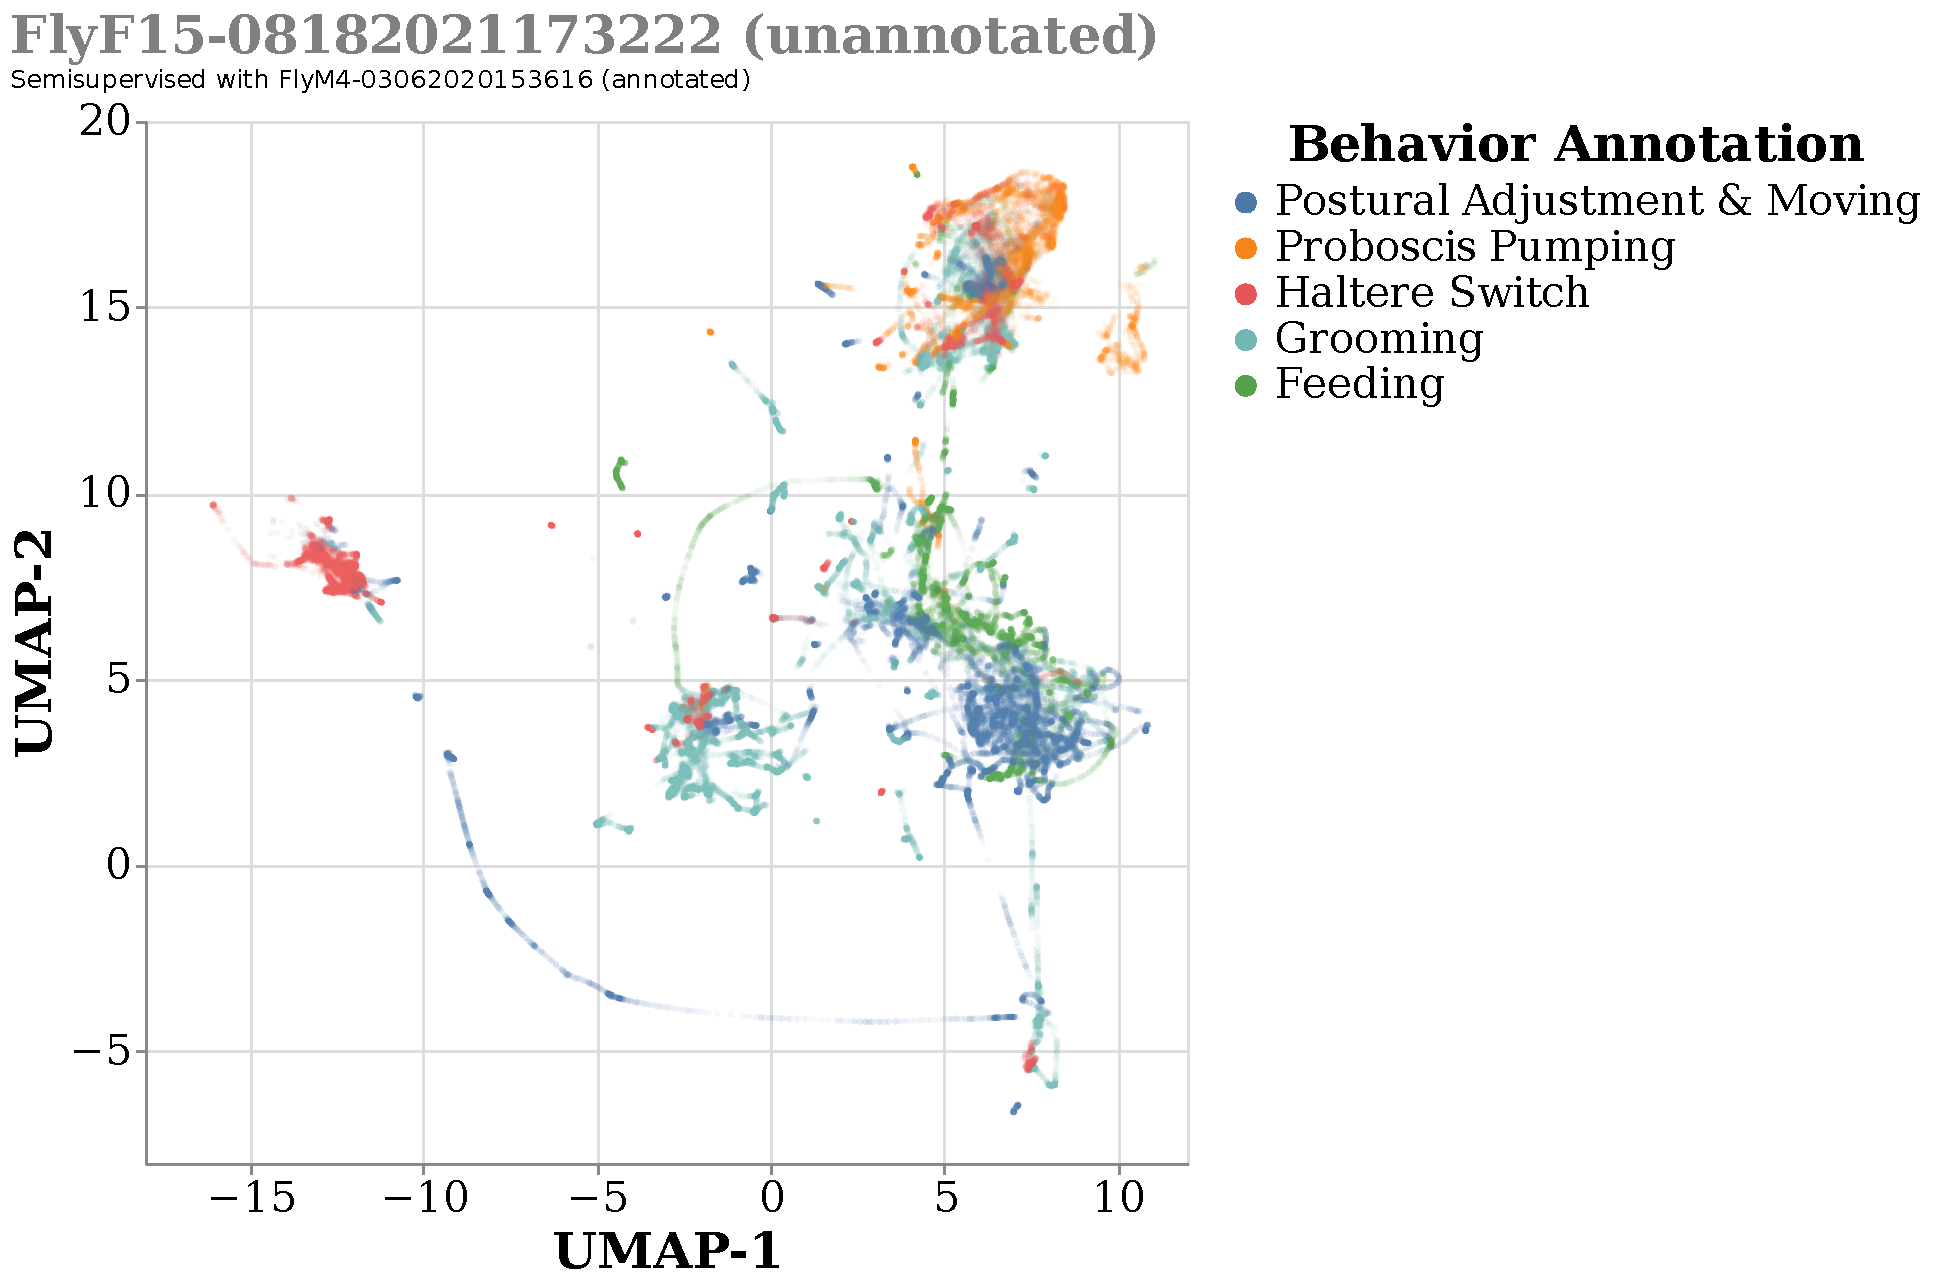
\includegraphics[height=5cm]{figures/FlyF15-08182021173222_FlyM4-03062020153616-SemisupervisedPairEmbedding.pdf}
		\caption{Only unannotated experiment.}
	\end{subfigure}%
	\hfill
	\centering
	\begin{subfigure}[b]{0.5\linewidth}
		\centering\includegraphics[height=5cm]{figures/FlyF15-08182021173222_FlyM4-03062020153616-SemisupervisedPairEmbedding-JointChart.pdf}
		\caption{Unannotated and annotated experiments.}
	\end{subfigure}%
	\caption[Semi-supervised pair embeddings with an annotated and an unannotated experiments.]{Semi-supervised pair embeddings with an annotated and an unannotated experiments. FlyM4-03062020 (annotated) provides a ``view'' on the behavioral repertoire of the FlyF15-08182021 (unannotated).}
\end{figure}

\begin{comment}
\section{Soft Clustering}
\citet{mcinnes_hdbscan_2017} \citet{campello_density-based_2013}
\NOTE{
	We always use soft clustering feature of HDBSCAN, since it is very beneficial to have a composite assignment for a data-point.
	For example, 0.7 grooming, 0.3 proboscis pumping may indicate that those two behaviors are simultaneously exhibited or a combination of both is exhibited etc.
	We can always take $\argmax$ if a categorical label is needed.
}

\subsection{Disparate Clustering}

\NOTE{
	If embedding is a disparate embedding, then we directly cluster each of them separately.
	If a joint embedding or pair embedding is clustered, then experiments need to be extracted from the embedding space first, and then they need to be clustered separately.
}

\subsection{Joint Clustering}
\NOTE{
	This is only applicable to joint and pair embeddings. We cluster all the experiments in the behavioral embedding together.
}

\subsection{Crosswise Clustering}
\NOTE{
	This is again only applicable to joint and pair embeddings.
	For joint embeddings, we exclude a subgroup of experiments.
	For pair embeddings, we exclude one of the pair experiments.
	Then rest of the embedding is clustered and clusters are formed.
	Finally, for each excluded embedding, soft cluster membership vectors are computed based on the formed clusters.
}

\subsection{Mapping Clusters to Behavioral Categories}
\NOTE{
	If a clustering contains annotated experiments, we map that clusters in that clustering to a behavioral composition as follows ({\it subject to change, there are couple of alternatives})
	\begin{equation}
		m_\alpha = \frac{\textnormal{number of frames with annotation }\alpha \textnormal{ in the cluster}}{\textnormal{total number of frames with annotation }\alpha}.
	\end{equation}
	So for each cluster, we end up with a vector $\mathbf{m}=(m_\alpha)$, represent it behavioral composition.
}
\NOTE{
	Behavioral score of unannotated experiment will be computed using clustering membership score and behavioral composition mapping of those clusters.
	For example, using semi-supervised pair embeddings and crosswise clustering; one can compute behavioral scores for a frame as follows;
	\begin{equation}
		y_\alpha = \sum_{c=0}^C m^c_\alpha
	\end{equation}
	where $C$ is the number of clusters, $\mathbf{m}^c$ is the behavioral composition of the cluster $c$.
	As a result, for each frame, we end up with a behavioral score vector $\mathbf{y}=(y_\alpha)$.
}
\end{comment}

\section{Nearest Neighbor Analysis and Classification}\label{section:nearest-neighbors-classification}
One of our ultimate goals is to annotate an experiment using already annotated ones.
In previous sections and chapters, we described feature extraction, experiment outlining, and computation of behavioral embeddings.
In this section, we describe a novel nearest neighbor based classification approach, which has to tackle following challenges:
\begin{itemize}
	\item sparsity of behavioral expressions,
	\item imbalanced distribution of behavioral categories,
	\item scarcity of annotated experiments, which are laborious to produce,
	\item variation between experiments.
\end{itemize}
Our approach consists of two steps, briefly stated as follows:
\begin{enumerate}
	\item computing behavioral weights of an unannotated experiment, using its semi-supervised pair embeddings for each annotated  experiment,
	\item combining behavioral weights of the unannotated experiment with an annotated experiment committee by voting.
\end{enumerate}
We compute the behavioral weights with our nearest neighbor based approach by considering sparsity of behavioral expressions and imbalanced distribution of behavioral categories, as described in Section~\ref{section:behavioral-weights}.
In the Section~\ref{section:committee-by-voting}, we detail the committee by voting approach, which helps us to deal with variation between experiments by providing multiple ``views'' on observed behavioral expression that we attempt to annotate. Finally, the post-processing of resulting predictions is described in the Section~\ref{section:postprocessing-predictions}.

\subsection{Behavioral Weights}\label{section:behavioral-weights}
Consider two experiments, an annotated one $\exptAnn$, and an unannotated one $\exptUnann$, and their semi-supervised pair embedding, respectively $\Ann{\V{E}}=\qmatrix{\Ann{\V{e}}_1, \cdots \Ann{\V{e}_{\Ann{F}}}}$ and $\Unann{\V{E}}=\qmatrix{\Unann{\V{e}}_1, \cdots \Unann{\V{e}}_{\Unann{F}}}$.
Given the true annotations $\Ann{\V{y}}$ of the frames in the $\Ann{\MicroActivity}$ set of $\exptAnn$, and $K$ behavioral categories, the goal is to compute $\V{\hat{b}}_f=\qmatrix{\hat{b}_{f,1}, \cdots \hat{b}_{f,K}}$, representing the weights (in other words, the similarity score) of each behavioral category for $\exptUnann$, using $\Ann{\V{E}}, \Unann{\V{E}}$ and $\Ann{\V{y}}$.

The procedure start by querying $k$-nearest neighbors of $\exptUnann$'s each frame $f$ in the joint behavioral embedding space consisting of $\Ann{\V{E}}$ and $\Unann{\V{E}}$, using the $k$-d trees for efficiency \citep{bentley_multidimensional_1975}. $\NN{k}{f}$ denotes the set of indices of $\Unann{\V{e}}_f$'s $k$ nearest neighbors, and the $k$-NN weight $b_{f,i}$ for each query point (i.e., frame) $f$ of $\exptUnann$, and behavioral category $i$, is computed by
\begin{equation}\label{equation:nn-weights}
	b_{f,i} = \begin{dcases}
		\sum_{f^\prime \in \NNi{k}{i}{f}}\frac{1}{\dist{\Unann{\V{e}}_f}{\Ann{\V{e}}_{f^\prime}}^p + \epsilon} & \textnormal{if } \card{\NNi{k}{i}{f}} \neq 0, \\
		0                                                                                                      & \textnormal{if otherwise},
	\end{dcases} \qbwhere p \in \set{0,1,2}.
\end{equation}
Here, $\NNi{k}{i}{f}=\Set{f^\prime}{\Ann{y}_{f^\prime}=i, \dband f^\prime \in \NN{k}{f}}$, is the set of indices of data points of $\exptAnn$ whose annotation is the behavior category $i$ and is one of the $k$ nearest neighbors of $\Unann{\V{e}}_f$.
$\dist{\Unann{\V{e}}_f}{\Ann{\V{e}}_{f^\prime}}$ is the euclidean distance between $\Unann{\V{e}}_f$ and $\Ann{\V{e}}_{f^\prime}$, and $p$ parameterizes the relation between distance and weight $b_{f,i}$.
We add a small number $\epsilon$ ($10^{{-}6}$) to the denominator to avoid numerical errors.
The resulting vector $\V{b}_f = \qmatrix{b_{f,1}, \cdots, b_{f,K}}$ weights the similarity of the frame $f$ to each behavioral category in the shared embedding space based on nearest neighbors.

Naturally, the number of occurrences or durations of the behavior bouts are different for each behavioral category, and therefore, $\Ann{\V{y}}$ is highly imbalanced.
As a result, number of nearest neighbors and $\V{b}_f$ are biased in favor of frequently occurring and long-bout behaviors.
For instance, pumping-like movements of the proboscis occur more frequently in longer bouts than switch-like movements of the haltere.
Especially when $k$ is large, it becomes crucial to consider the imbalanced distribution of behavior occurrences, since the embedding space will be dominated by frequent behaviors.
Thus, incorporating this imbalance into the formulation may help to improve the recall of rarely occurring short-bout behaviors and precision of frequently occurring long-bout behaviors.
To achieve this, we normalize the scores previously computed, $b_{f,i}$, as a function of the number of occurrences of the behavioral category $i$ as follows:

\begin{equation}\label{equation:behavioral-weight-occurence-normalization},
	b^\prime_{f,i} = \frac{b_{f,i}}{\rbr{1 + N^{\plus}_i}^p} \qbor \frac{b_{f,i}}{\log_k(1 + N^{\plus}_i)} \qbwhere p \in \set{0, \sfrac{1}{2}, 1}, k \in \set{2, 10},
\end{equation}
where $N^{\plus}_i = \card*{\Set{f}{y^{\plus}_f=i}}$ is the number of frames annotated as behavioral category $i$.
In the above equation, two different alternatives are given for this normalization step; a polynomial one and a logarithmic one, where $p$ and $k$ parameterize the relation between $N^{\plus}_i$ and $b^\prime_{f,i}$.
For instance, if one is mostly interested in achieving high recall for frequently occurring behaviors, low $p$ values or using the logarithmic alternative might be more appropriate.
It may be even desired to set $p=0$, and not considering the number of occurrences in some cases, see Section~\ref{section:employing-proposed-pipeline} for more details.

The resulting vector $\V{b^{\prime}}_f \in \reals^K$ is dependent on the annotated experiment $\exptAnn$, and the vectors computed based on different annotated experiments are not comparable with each other.
Hence, we map the values of $b^\prime_{f,i}$ to $\sqbr{0,1}$ using either the $\operatorname {softmax}$ function or $\textnormal{L}_1$ normalization as follows:
\begin{equation}\label{equation:behavioral-weight-activation}
	\hat{b}_{f,i} = \frac{\exp{b^\prime_{f,i}}}{\sum_{j=1}^{K} \exp{b^\prime_{f,j}}} \qbor \frac{b^\prime_{f,i}}{\sum_{j=1}^{K} b^\prime_{f,j}}.
\end{equation}
The resulting behavioral weight vector $\V{\hat{b}}_f \in \sqbr{0,1}^K$ can be considered as a probability distribution.
Here, the vector $\V{\hat{b}}_f$ represents the behavioral characteristics of the frame $f$ of $\exptUnann$ based on the behavioral repertoire of $\exptAnn$.
The voting-like scheme, as described in Section~\ref{section:committee-by-voting}, incorporates the behavioral weight vectors of all annotated experiments to finalize the classification for $\exptUnann$.

\subsection{Experiment Committee by Voting}\label{section:committee-by-voting}
Consider all experiments: unannotated experiments $\exptUnann_1, \cdots, \exptUnann_{\Unann{R}}$, and annotated experiments $\exptAnn_1, \cdots, \exptAnn_{\Ann{R}}$, where $\Unann{R}$ and $\Ann{R}$ are the number of experiments, respectively.
The goal is to combine the behavioral weights of an unannotated experiment $\exptUnann_k$, calculated separately for each annotated experiment.

Let $\V{\hat{b}}_f^{k,l}$ denote the behavioral weights of $\exptUnann_k$ computed with $\exptAnn_l$.
Each annotated experiment contributes to the overall behavioral score of $\exptUnann_k$; in other words, annotated experiments, forming a committee,  vote according to $\V{\hat{b}}_f^{k,l}$.
Each annotated experiment provides a different view to the behavioral repertoire, as in the case of pair embeddings (see Section~\ref{section:pair-embeddings}).
Before describing hard voting and soft voting approaches, there is one more step to discuss.

There exists a significant variation among the exhibited behavioral repertoires in the experiments.
An annotated experiment might lack some behavioral expressions or manifest some behaviors excessively.
In such cases, if the behavioral weight vector $\V{\hat{b}}_f^{k,l}$ is not confident, i.e., weights of behavioral categories are close to each other, one may want to decrease its contribution to the voting.
To achieve this, we propose two optional approaches; penalizing the behavioral weights with the entropy of the ``probability distribution'' $\V{\hat{b}}_f^{k,l}$, or with the uncertainty.
The contribution of votes of $\exptAnn_l$ to the committee formed for $\exptUnann_k$ is $\Vvote_f^{k,l} = \qmatrix{\vote_{f,1}^{k,l}, \cdots, \vote_{f,K}^{k,l}}$, and is given by
\begin{equation}
	\vote_{f,i}^{k,l} = \rbr{\log_2(K) - \entropy{\V{\hat{b}}_f^{k,l}}} \hat{b}_{f,i}^{k,l} \qbor \rbr{ 1 - \max_{1 \leq j \leq K} \hat{b}_{f,j}^{k,l}} \hat{b}_{f,i}^{k,l} \qbor \hat{b}_{f,i}^{k,l}.
\end{equation}
If $\max_i \hat{b}_{f,i}$ is close to $\sfrac{1}{K}$, which means that the computed vector weights the behaviors uniformly, then the factors $\rbr{\log_2(K) - \entropy{\V{\hat{b}}_f^{k,l}}}$ or $\rbr{ 1 - \max_{1 \leq j \leq K} \hat{b}_{f,j}^{k,l}}$ may be used to decrease the ``importance'' of the vote.

Now, after computing behavioral votes for each annotated and unannotated experiment pair, we can combine those votes for a single unannotated experiment $\exptUnann_k$  by forming a committee of annotated experiments $\exptAnn_1, \cdots, \exptAnn_{\Ann{R}}$.
The predicted behavioral category at frame $k$ of $\exptUnann_k$ is given by combined votes of the committee.
The predicted behavioral category at frame $k$ of $\exptUnann_k$, denoted by $\hat{y}^k_f$, is given by combined votes of the committee.
To obtain the overall aggregate view of the committee, we can follow two alternative voting schemes, namely hard voting (i.e., majority rule voting) or soft voting.
At this point, we may want to have scores for each behavioral category rather than hard-labels.
Such score information might be desired to capture complex and hierarchical structure of the behaviors.
Behaviors sometimes occur simultaneously, and sometimes observed behaviors might manifest similarities to more than one behavioral category \citep{berman_predictability_2016}.
Hence, one may also use the combined vote scores directly, without computing the $\argmax$.

\subsubsection{Hard Voting}
In the hard voting scheme, prediction of a frame $f$ is given by the majority behavioral category of the $\argmax$ of the each annotated experiment's votes and computed by the following formula:
\begin{equation}
	\hat{y}^k_f = \argmax_{1 \leq i \leq K} \Set{\argmax_{1 \leq j \leq K} { \vote_{f,j}^{k,l}}}{j=i, \, 1 \leq l \leq \Ann{R}}.
\end{equation}

\subsubsection{Soft Voting}
In contrast to majority voting (hard voting), the soft voting scheme assigns the behavioral category as the $\argmax$ of the sum of each annotated experiment's vote vector, and $\hat{y}^k_f$ is given by
\begin{equation}
	\hat{y}^k_f = \argmax_{1 \leq i \leq K} \sum_{l=1}^{\Ann{R}} \vote_{f,i}^{k,l}.
\end{equation}

\subsubsection{Behavioral Scores}
Definitions of behavioral categories might be broad, and expressed behaviors sometimes are a combination of multiple behavioral categories.
For example a switch-like movement of the haltere can simultaneously occur with a postural adjustment.
Also, one may also want to examine and interpret top-$k$ predictions, especially when there exists many narrow behavioral categories.
Thus, in addition to assigning categories to frames, it is also useful to compute and report scores for behavioral category based on the votes contributed by each annotated experiments.
Moreover, such scores can be utilized as confidence scores, and might be helpful to analyze differences in behavioral repertoire (see Figure~\ref{figure:behavioral-score-distributions} and Figure~\ref{figure:repertoire-difference}).

For a behavioral category $i$, such a score can be calculated by combining votes as follows:
\begin{equation}
	\frac{\sum_{l=1}^{\Ann{R}} \vote_{f,i}^{k,l}}{\sum_{i = 1}^{K}\sum_{l=1}^{\Ann{R}} \vote_{f,i}^{k,l}}.
\end{equation}

\subsection{Post-processing}\label{section:postprocessing-predictions}
Finally, we post-process predicted annotations to improve our nearest neighbor based algorithm by incorporating a couple of assumptions on the temporal organization of the behaviors and physical constrains.
Before applying post-processing procedures, the frames in the sets $\MacroActivity$ and $\Quiescence$ should be recovered, as we only predicted the annotations of the frames in the set $\MicroActivity$.
Without having a temporally continuous vector of annotations, post-processing would lead unintended consequences and erroneous results.
Let $\VpredAnn^k=\rbr{\hat{y}^k_1, \cdots, \hat{y}^k_T}$ be the $\exptUnann_k$'s vector of predicted annotations for the entire experiment, defined as follows:
\begin{equation}
	\predAnn^k_t =
	\begin{cases}
		0           & \textnormal{if } t \in \Quiescence_k,                             \\
		\hat{y}^k_f & \textnormal{if } t \in \MicroActivity_k \textnormal{ and } t=t_f, \\
		K+1         & \textnormal{if } t \in \MacroActivity_k.
	\end{cases}
\end{equation}
This vector of annotations spans an entire experiment of $k$, and consists of detailed annotations of behavioral subcategories during dormancy, the general category of macro-activities, and quiescence.

Before discussing the post-processing, we first need to define behavioral bouts.
Informally, a behavioral bout is a segment of time, in which the same behavioral category is continuously observed.
We can formally define a behavioral bout for a given $\hat{y}^k_t$ as follows:
\begin{equation}
	\begin{aligned}
		\mathsf{bout}^0_t & =\max\cbr{{\argmax_{t^\prime} \rbr{\hat{y}^k_t \neq \hat{y}^k_{t^\prime}} \land \rbr{1 \leq t^\prime \leq t} \lor \rbr{t^\prime = 1}}}, \\
		\mathsf{bout}^1_t & =\min\cbr{{\argmax_{t^\prime} \rbr{\hat{y}^k_t \neq \hat{y}^k_{t^\prime}} \land \rbr{t \leq t^\prime \leq T} \lor \rbr{t^\prime = T}}},
	\end{aligned}
\end{equation}
where $\mathsf{bout}^0_t$ and $\mathsf{bout}^1_t$ are respectively the beginning and the end of the behavioral bout, which $\hat{y}^k_t$ belongs to.

We have sensible expectations about the durations of behavioral bouts of each behavioral category acquired by human annotators.
For instance, a bout of proboscis's pumping-like movement should not be shorter than $200$ millisecond, as bout duration distributions of annotations indicates.
In addition to annotations, we may have reason about physical and biological constraints.
An example is that grooming behavior, bout duration of grooming can not exceed a couple of minutes, probability of observing a grooming behavior lasted longer than $2$ minutes is extremely low \citep{qiao_automated_2018}.
Considering such constraints and temporal expectations, we apply the following post-processing procedures, and parameters should be determined based on the behavioral repertoire of interest.
Post-processing procedures are especially helpful for avoiding misleading classification of the time points with erroneous tracking of body parts.
Each procedure is optional, but should be applied in the given order.

\subsubsection{Pruning Interrupting Bouts}\label{section:pruning-interrupting-bouts}
We prune short intervals interrupting possibly long and continuous behavioral bouts.
Given a window size $\tau$, the majority behavioral category in the surrounding window around a time point $t$ is assigned that point by:
\begin{equation}
	\hat{\predAnn^k_t} = \argmax_{\symsf{a}} \card{\Set{t^\prime}{\predAnn^k_{t^\prime}=\symsf{a}, \ \max\cbr{1, t-\tau} \leq t^\prime \leq \min\cbr{t+\tau, T}}}.
\end{equation}
The window size $\tau$ is typically less than a second.

\subsubsection{Elimination of Overly Long and Overly Short Bouts}
We eliminate behavioral bouts whose durations are extremely short or extremely long, and hence, contradicting with physical constraints and our temporal expectations.
For each behavioral category $i$, we define two thresholds $\delta^{\symrm{short}}_i$ and $\delta^{\symrm{long}}_i$, namely upper bound and lower bound.
Then, the behavioral bouts whose duration longer or shorter than the corresponding thresholds, are set to quiescence.
\begin{equation}
	\hat{\predAnn}^k_t=
	\begin{cases}
		0            & \mathsf{bout}^0_t - \mathsf{bout}^1_t < \delta^{\symrm{short}}_{\predAnn^k_t}, \\
		0            & \mathsf{bout}^0_t - \mathsf{bout}^1_t > \delta^{\symrm{long}}_{\predAnn^k_t},  \\
		\predAnn^k_t & \textnormal{otherwise},
	\end{cases}
\end{equation}
For each behavioral category $i$, the thresholds $\delta^{\symrm{short}}_i$ ($\delta^{\symrm{long}}_i$) should be greater (smaller) than the window size $\tau$ used in Section~\ref{section:pruning-interrupting-bouts}.
